% How the evolution MPO is built from the Hamiltonian FSM (Appendix app:mpo:vd2).
% (a) first order: the closing level is folded back onto the start with a factor tau.
% (b) second order: the same move applied to H^2, whose levels are pairs of levels.
%
% Standalone: compiles on its own to imgs/vd2_folding.pdf.
% Inline:     with \usepackage{standalone} in the preamble, % How the evolution MPO is built from the Hamiltonian FSM (Appendix app:mpo:vd2).
% (a) first order: the closing level is folded back onto the start with a factor tau.
% (b) second order: the same move applied to H^2, whose levels are pairs of levels.
%
% Standalone: compiles on its own to imgs/vd2_folding.pdf.
% Inline:     with \usepackage{standalone} in the preamble, % How the evolution MPO is built from the Hamiltonian FSM (Appendix app:mpo:vd2).
% (a) first order: the closing level is folded back onto the start with a factor tau.
% (b) second order: the same move applied to H^2, whose levels are pairs of levels.
%
% Standalone: compiles on its own to imgs/vd2_folding.pdf.
% Inline:     with \usepackage{standalone} in the preamble, % How the evolution MPO is built from the Hamiltonian FSM (Appendix app:mpo:vd2).
% (a) first order: the closing level is folded back onto the start with a factor tau.
% (b) second order: the same move applied to H^2, whose levels are pairs of levels.
%
% Standalone: compiles on its own to imgs/vd2_folding.pdf.
% Inline:     with \usepackage{standalone} in the preamble, \input{imgs/vd2_folding} drops it in.
\documentclass[tikz,border=3pt]{standalone}
\usepackage{amsmath,amssymb,bbold}
\usetikzlibrary{automata,arrows.meta,positioning,calc}

\newcommand{\ident}{\mathbb{1}}

\begin{document}
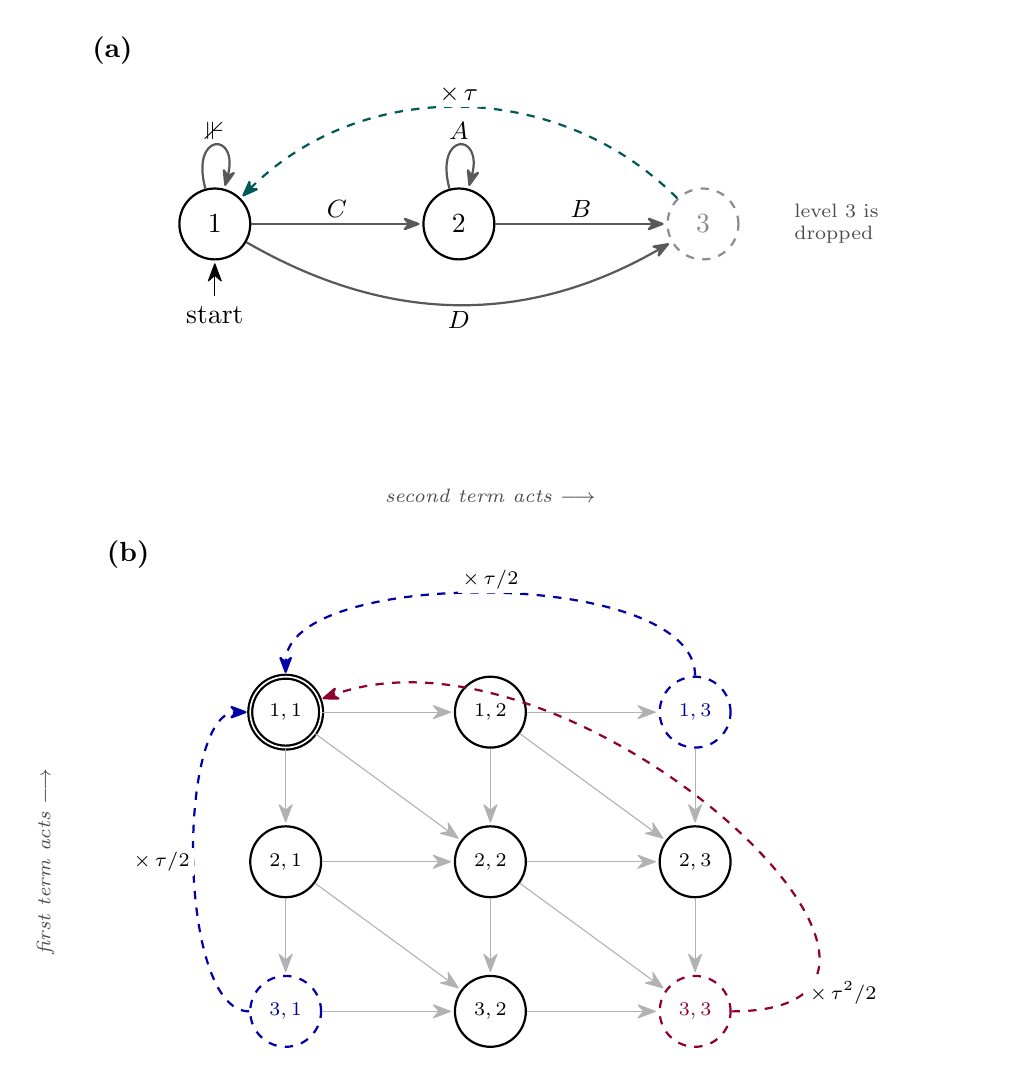
\begin{tikzpicture}[
    >={Stealth[round,length=2.6mm]},
    shorten >=1pt,
    state/.style={circle, draw, thick, minimum size=9mm, inner sep=1pt},
    gone/.style={circle, draw, thick, dashed, draw=black!45, text=black!45,
                 minimum size=9mm, inner sep=1pt},
    pair/.style={circle, draw, thick, minimum size=9mm, inner sep=0pt, font=\scriptsize},
    discnode/.style={circle, draw, thick, dashed, draw=blue!65!black, text=blue!65!black,
                     minimum size=9mm, inner sep=0pt, font=\scriptsize},
    connode/.style={circle, draw, thick, dashed, draw=purple!75!black, text=purple!75!black,
                    minimum size=9mm, inner sep=0pt, font=\scriptsize},
    lbl/.style={font=\small, inner sep=2pt},
    slbl/.style={font=\scriptsize, inner sep=1.5pt},
    hdr/.style={font=\scriptsize\itshape, text=black!70},
    plain/.style={draw=black!65, ->, thick},
    advance/.style={draw=black!30, ->, thin},
    fold/.style={draw=teal!70!black, ->, thick, dashed},
    disc/.style={draw=blue!65!black, ->, thick, dashed},
    conn/.style={draw=purple!75!black, ->, thick, dashed},
    panel/.style={font=\bfseries},
  ]

  %% ---------------------------------------------------------------- panel (a)
  \node[panel] at (-1.3,2.2) {(a)};

  \node[state, initial below, initial text={start}] (a1) at (0,0)   {$1$};
  \node[state]                                      (a2) at (3.1,0) {$2$};
  \node[gone]                                       (a3) at (6.2,0) {$3$};

  \path (a1) edge[plain, loop above] node[lbl, above] {$\ident$} (a1);
  \path (a2) edge[plain, loop above] node[lbl, above] {$A$}      (a2);
  \path (a1) edge[plain]                node[lbl, above] {$C$} (a2);
  \path (a2) edge[plain]                node[lbl, above] {$B$} (a3);
  \path (a1) edge[plain, bend right=30] node[lbl, below] {$D$} (a3);

  % the one move that turns the Hamiltonian machine into an evolution operator
  \path (a3) edge[fold, bend right=45]
        node[lbl, above, pos=0.5, fill=white, inner sep=1.5pt] {$\times\,\tau$} (a1);

  \node[slbl, text=black!70, anchor=west] at (7.3,0)
       {\begin{tabular}{@{}l@{}}level $3$ is\\dropped\end{tabular}};

  %% ---------------------------------------------------------------- panel (b)
  \begin{scope}[yshift=-6.2cm, xshift=0.9cm]
    \node[panel] at (-2.0,2.0) {(b)};

    % 3x3 grid of pair levels: (row, column) = (state of first term, state of second term)
    \node[pair, double, double distance=0.6pt] (q11) at (0,0) {$1,1$};
    \node[pair]     (q12) at (2.6,0)    {$1,2$};
    \node[discnode] (q13) at (5.2,0)    {$1,3$};
    \node[pair]     (q21) at (0,-1.9)   {$2,1$};
    \node[pair]     (q22) at (2.6,-1.9) {$2,2$};
    \node[pair]     (q23) at (5.2,-1.9) {$2,3$};
    \node[discnode] (q31) at (0,-3.8)   {$3,1$};
    \node[pair]     (q32) at (2.6,-3.8) {$3,2$};
    \node[connode]  (q33) at (5.2,-3.8) {$3,3$};

    % which index is which
    \node[hdr] at (2.6,2.75) {second term acts $\longrightarrow$};
    \node[hdr, rotate=90] at (-3.05,-1.9) {first term acts $\longrightarrow$};
    

    % Either index may advance on its own (right, down) or both at the same site (diagonal).
    \foreach \r in {1,2,3}{
      \path (q\r1) edge[advance] (q\r2);
      \path (q\r2) edge[advance] (q\r3);
    }
    \foreach \c in {1,2,3}{
      \path (q1\c) edge[advance] (q2\c);
      \path (q2\c) edge[advance] (q3\c);
    }
    \path (q11) edge[advance] (q22);
    \path (q12) edge[advance] (q23);
    \path (q21) edge[advance] (q32);
    \path (q22) edge[advance] (q33);

    % One term finished while the other never started: a disjoint pair. Both folds are routed
    % outside the grid so they never cross a node.
    \draw[disc] (q13) to[out=90, in=90, looseness=0.68]
      node[slbl, above, pos=0.5, fill=white, inner sep=1.5pt] {$\times\,\tau/2$} (q11);
    \draw[disc] (q31) to[out=180, in=180, looseness=0.62]
      node[slbl, left, pos=0.5, fill=white, inner sep=1.5pt] {$\times\,\tau/2$} (q11);
    % With those removed, this level is reachable only through overlapping terms.
    \draw[conn] (q33) to[out=0, in=20, looseness=1.35]
      node[slbl, right, pos=0.13, fill=white, inner sep=1.5pt] {$\times\,\tau^{2}/2$} (q11);
  \end{scope}

\end{tikzpicture}
\end{document}
 drops it in.
\documentclass[tikz,border=3pt]{standalone}
\usepackage{amsmath,amssymb,bbold}
\usetikzlibrary{automata,arrows.meta,positioning,calc}

\newcommand{\ident}{\mathbb{1}}

\begin{document}
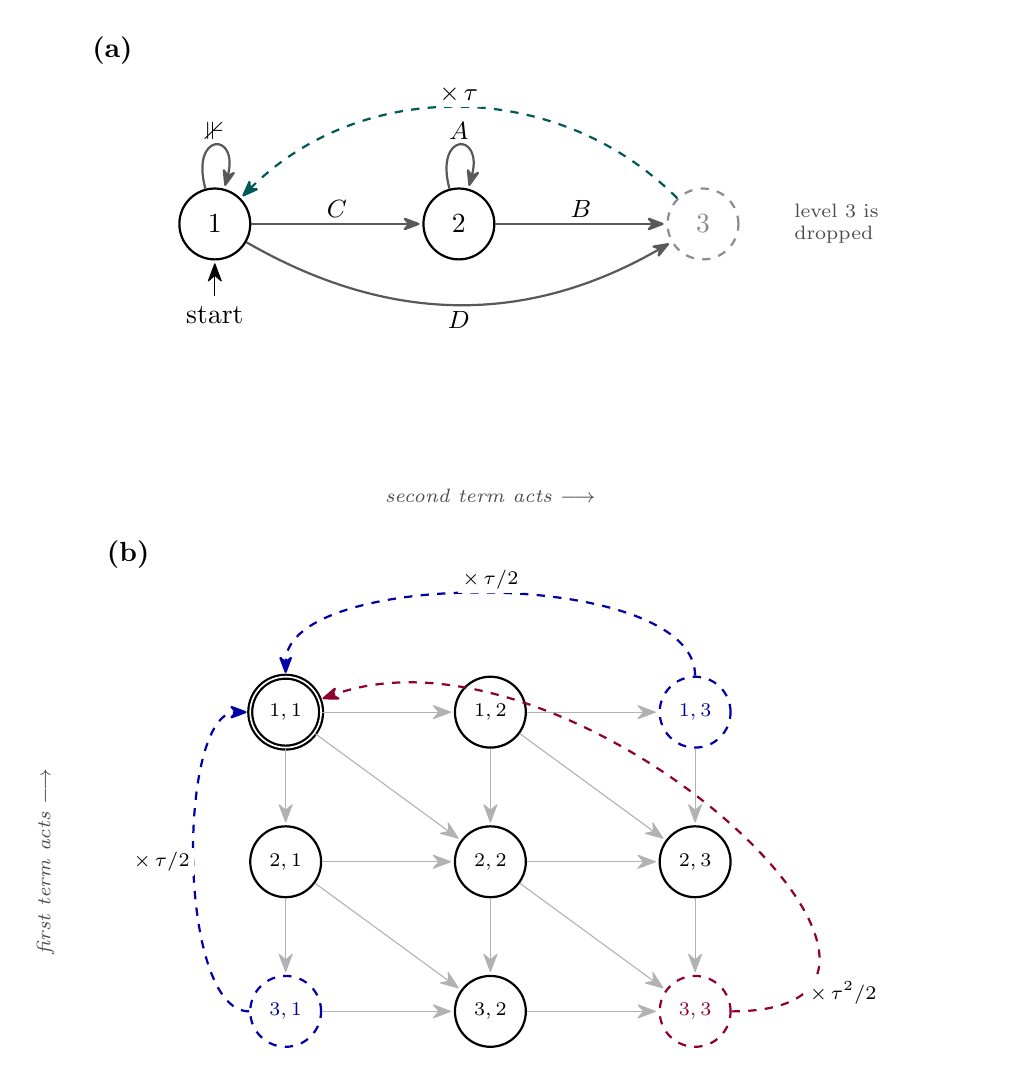
\begin{tikzpicture}[
    >={Stealth[round,length=2.6mm]},
    shorten >=1pt,
    state/.style={circle, draw, thick, minimum size=9mm, inner sep=1pt},
    gone/.style={circle, draw, thick, dashed, draw=black!45, text=black!45,
                 minimum size=9mm, inner sep=1pt},
    pair/.style={circle, draw, thick, minimum size=9mm, inner sep=0pt, font=\scriptsize},
    discnode/.style={circle, draw, thick, dashed, draw=blue!65!black, text=blue!65!black,
                     minimum size=9mm, inner sep=0pt, font=\scriptsize},
    connode/.style={circle, draw, thick, dashed, draw=purple!75!black, text=purple!75!black,
                    minimum size=9mm, inner sep=0pt, font=\scriptsize},
    lbl/.style={font=\small, inner sep=2pt},
    slbl/.style={font=\scriptsize, inner sep=1.5pt},
    hdr/.style={font=\scriptsize\itshape, text=black!70},
    plain/.style={draw=black!65, ->, thick},
    advance/.style={draw=black!30, ->, thin},
    fold/.style={draw=teal!70!black, ->, thick, dashed},
    disc/.style={draw=blue!65!black, ->, thick, dashed},
    conn/.style={draw=purple!75!black, ->, thick, dashed},
    panel/.style={font=\bfseries},
  ]

  %% ---------------------------------------------------------------- panel (a)
  \node[panel] at (-1.3,2.2) {(a)};

  \node[state, initial below, initial text={start}] (a1) at (0,0)   {$1$};
  \node[state]                                      (a2) at (3.1,0) {$2$};
  \node[gone]                                       (a3) at (6.2,0) {$3$};

  \path (a1) edge[plain, loop above] node[lbl, above] {$\ident$} (a1);
  \path (a2) edge[plain, loop above] node[lbl, above] {$A$}      (a2);
  \path (a1) edge[plain]                node[lbl, above] {$C$} (a2);
  \path (a2) edge[plain]                node[lbl, above] {$B$} (a3);
  \path (a1) edge[plain, bend right=30] node[lbl, below] {$D$} (a3);

  % the one move that turns the Hamiltonian machine into an evolution operator
  \path (a3) edge[fold, bend right=45]
        node[lbl, above, pos=0.5, fill=white, inner sep=1.5pt] {$\times\,\tau$} (a1);

  \node[slbl, text=black!70, anchor=west] at (7.3,0)
       {\begin{tabular}{@{}l@{}}level $3$ is\\dropped\end{tabular}};

  %% ---------------------------------------------------------------- panel (b)
  \begin{scope}[yshift=-6.2cm, xshift=0.9cm]
    \node[panel] at (-2.0,2.0) {(b)};

    % 3x3 grid of pair levels: (row, column) = (state of first term, state of second term)
    \node[pair, double, double distance=0.6pt] (q11) at (0,0) {$1,1$};
    \node[pair]     (q12) at (2.6,0)    {$1,2$};
    \node[discnode] (q13) at (5.2,0)    {$1,3$};
    \node[pair]     (q21) at (0,-1.9)   {$2,1$};
    \node[pair]     (q22) at (2.6,-1.9) {$2,2$};
    \node[pair]     (q23) at (5.2,-1.9) {$2,3$};
    \node[discnode] (q31) at (0,-3.8)   {$3,1$};
    \node[pair]     (q32) at (2.6,-3.8) {$3,2$};
    \node[connode]  (q33) at (5.2,-3.8) {$3,3$};

    % which index is which
    \node[hdr] at (2.6,2.75) {second term acts $\longrightarrow$};
    \node[hdr, rotate=90] at (-3.05,-1.9) {first term acts $\longrightarrow$};
    

    % Either index may advance on its own (right, down) or both at the same site (diagonal).
    \foreach \r in {1,2,3}{
      \path (q\r1) edge[advance] (q\r2);
      \path (q\r2) edge[advance] (q\r3);
    }
    \foreach \c in {1,2,3}{
      \path (q1\c) edge[advance] (q2\c);
      \path (q2\c) edge[advance] (q3\c);
    }
    \path (q11) edge[advance] (q22);
    \path (q12) edge[advance] (q23);
    \path (q21) edge[advance] (q32);
    \path (q22) edge[advance] (q33);

    % One term finished while the other never started: a disjoint pair. Both folds are routed
    % outside the grid so they never cross a node.
    \draw[disc] (q13) to[out=90, in=90, looseness=0.68]
      node[slbl, above, pos=0.5, fill=white, inner sep=1.5pt] {$\times\,\tau/2$} (q11);
    \draw[disc] (q31) to[out=180, in=180, looseness=0.62]
      node[slbl, left, pos=0.5, fill=white, inner sep=1.5pt] {$\times\,\tau/2$} (q11);
    % With those removed, this level is reachable only through overlapping terms.
    \draw[conn] (q33) to[out=0, in=20, looseness=1.35]
      node[slbl, right, pos=0.13, fill=white, inner sep=1.5pt] {$\times\,\tau^{2}/2$} (q11);
  \end{scope}

\end{tikzpicture}
\end{document}
 drops it in.
\documentclass[tikz,border=3pt]{standalone}
\usepackage{amsmath,amssymb,bbold}
\usetikzlibrary{automata,arrows.meta,positioning,calc}

\newcommand{\ident}{\mathbb{1}}

\begin{document}
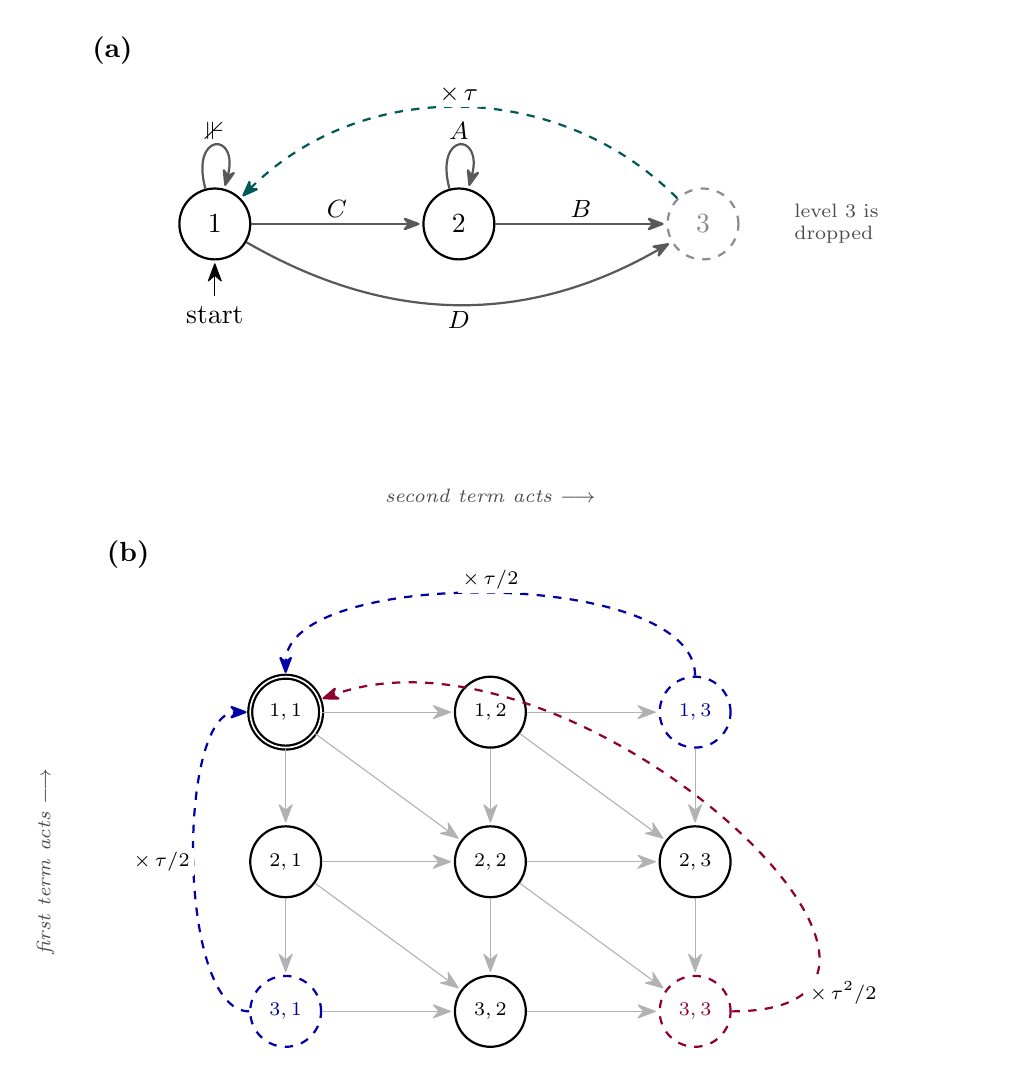
\begin{tikzpicture}[
    >={Stealth[round,length=2.6mm]},
    shorten >=1pt,
    state/.style={circle, draw, thick, minimum size=9mm, inner sep=1pt},
    gone/.style={circle, draw, thick, dashed, draw=black!45, text=black!45,
                 minimum size=9mm, inner sep=1pt},
    pair/.style={circle, draw, thick, minimum size=9mm, inner sep=0pt, font=\scriptsize},
    discnode/.style={circle, draw, thick, dashed, draw=blue!65!black, text=blue!65!black,
                     minimum size=9mm, inner sep=0pt, font=\scriptsize},
    connode/.style={circle, draw, thick, dashed, draw=purple!75!black, text=purple!75!black,
                    minimum size=9mm, inner sep=0pt, font=\scriptsize},
    lbl/.style={font=\small, inner sep=2pt},
    slbl/.style={font=\scriptsize, inner sep=1.5pt},
    hdr/.style={font=\scriptsize\itshape, text=black!70},
    plain/.style={draw=black!65, ->, thick},
    advance/.style={draw=black!30, ->, thin},
    fold/.style={draw=teal!70!black, ->, thick, dashed},
    disc/.style={draw=blue!65!black, ->, thick, dashed},
    conn/.style={draw=purple!75!black, ->, thick, dashed},
    panel/.style={font=\bfseries},
  ]

  %% ---------------------------------------------------------------- panel (a)
  \node[panel] at (-1.3,2.2) {(a)};

  \node[state, initial below, initial text={start}] (a1) at (0,0)   {$1$};
  \node[state]                                      (a2) at (3.1,0) {$2$};
  \node[gone]                                       (a3) at (6.2,0) {$3$};

  \path (a1) edge[plain, loop above] node[lbl, above] {$\ident$} (a1);
  \path (a2) edge[plain, loop above] node[lbl, above] {$A$}      (a2);
  \path (a1) edge[plain]                node[lbl, above] {$C$} (a2);
  \path (a2) edge[plain]                node[lbl, above] {$B$} (a3);
  \path (a1) edge[plain, bend right=30] node[lbl, below] {$D$} (a3);

  % the one move that turns the Hamiltonian machine into an evolution operator
  \path (a3) edge[fold, bend right=45]
        node[lbl, above, pos=0.5, fill=white, inner sep=1.5pt] {$\times\,\tau$} (a1);

  \node[slbl, text=black!70, anchor=west] at (7.3,0)
       {\begin{tabular}{@{}l@{}}level $3$ is\\dropped\end{tabular}};

  %% ---------------------------------------------------------------- panel (b)
  \begin{scope}[yshift=-6.2cm, xshift=0.9cm]
    \node[panel] at (-2.0,2.0) {(b)};

    % 3x3 grid of pair levels: (row, column) = (state of first term, state of second term)
    \node[pair, double, double distance=0.6pt] (q11) at (0,0) {$1,1$};
    \node[pair]     (q12) at (2.6,0)    {$1,2$};
    \node[discnode] (q13) at (5.2,0)    {$1,3$};
    \node[pair]     (q21) at (0,-1.9)   {$2,1$};
    \node[pair]     (q22) at (2.6,-1.9) {$2,2$};
    \node[pair]     (q23) at (5.2,-1.9) {$2,3$};
    \node[discnode] (q31) at (0,-3.8)   {$3,1$};
    \node[pair]     (q32) at (2.6,-3.8) {$3,2$};
    \node[connode]  (q33) at (5.2,-3.8) {$3,3$};

    % which index is which
    \node[hdr] at (2.6,2.75) {second term acts $\longrightarrow$};
    \node[hdr, rotate=90] at (-3.05,-1.9) {first term acts $\longrightarrow$};
    

    % Either index may advance on its own (right, down) or both at the same site (diagonal).
    \foreach \r in {1,2,3}{
      \path (q\r1) edge[advance] (q\r2);
      \path (q\r2) edge[advance] (q\r3);
    }
    \foreach \c in {1,2,3}{
      \path (q1\c) edge[advance] (q2\c);
      \path (q2\c) edge[advance] (q3\c);
    }
    \path (q11) edge[advance] (q22);
    \path (q12) edge[advance] (q23);
    \path (q21) edge[advance] (q32);
    \path (q22) edge[advance] (q33);

    % One term finished while the other never started: a disjoint pair. Both folds are routed
    % outside the grid so they never cross a node.
    \draw[disc] (q13) to[out=90, in=90, looseness=0.68]
      node[slbl, above, pos=0.5, fill=white, inner sep=1.5pt] {$\times\,\tau/2$} (q11);
    \draw[disc] (q31) to[out=180, in=180, looseness=0.62]
      node[slbl, left, pos=0.5, fill=white, inner sep=1.5pt] {$\times\,\tau/2$} (q11);
    % With those removed, this level is reachable only through overlapping terms.
    \draw[conn] (q33) to[out=0, in=20, looseness=1.35]
      node[slbl, right, pos=0.13, fill=white, inner sep=1.5pt] {$\times\,\tau^{2}/2$} (q11);
  \end{scope}

\end{tikzpicture}
\end{document}
 drops it in.
\documentclass[tikz,border=3pt]{standalone}
\usepackage{amsmath,amssymb,bbold}
\usetikzlibrary{automata,arrows.meta,positioning,calc}

\newcommand{\ident}{\mathbb{1}}

\begin{document}
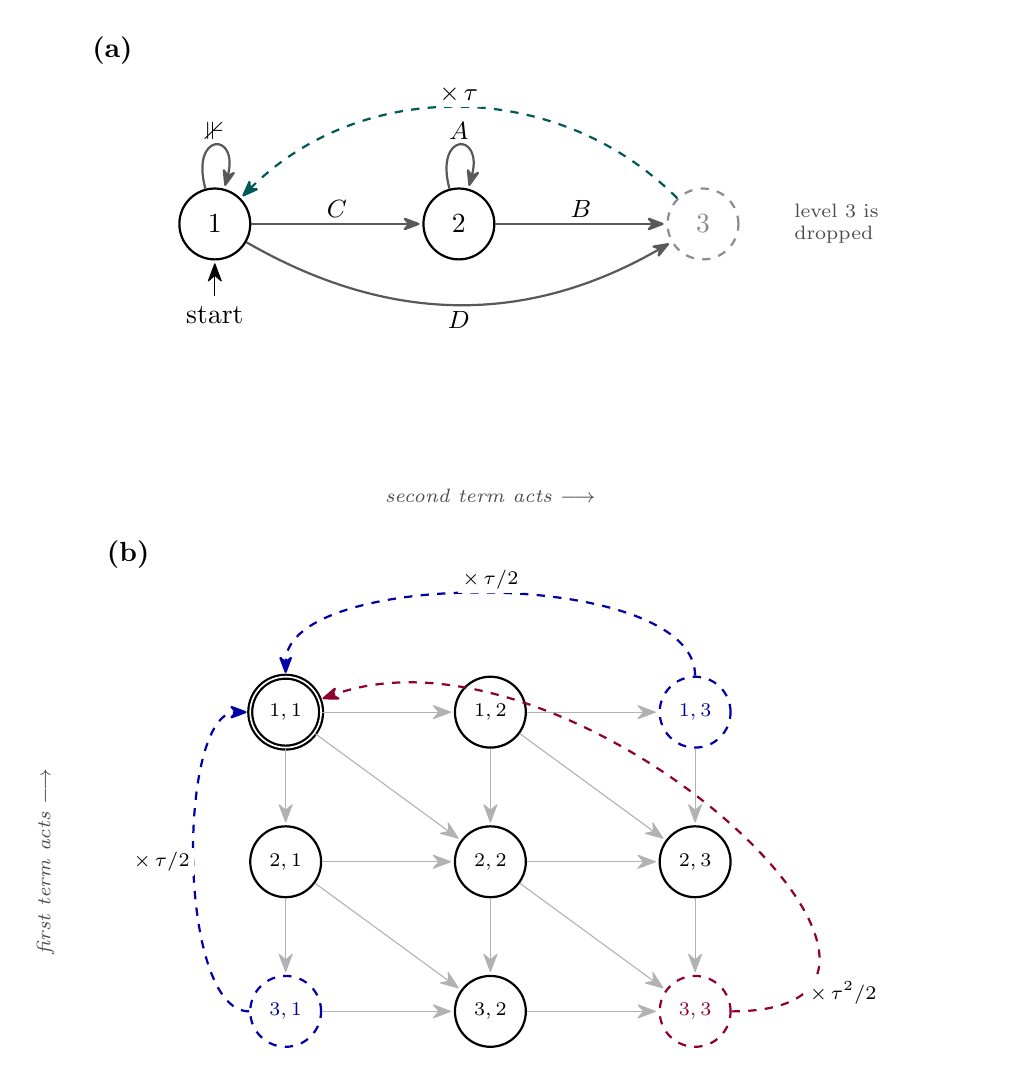
\begin{tikzpicture}[
    >={Stealth[round,length=2.6mm]},
    shorten >=1pt,
    state/.style={circle, draw, thick, minimum size=9mm, inner sep=1pt},
    gone/.style={circle, draw, thick, dashed, draw=black!45, text=black!45,
                 minimum size=9mm, inner sep=1pt},
    pair/.style={circle, draw, thick, minimum size=9mm, inner sep=0pt, font=\scriptsize},
    discnode/.style={circle, draw, thick, dashed, draw=blue!65!black, text=blue!65!black,
                     minimum size=9mm, inner sep=0pt, font=\scriptsize},
    connode/.style={circle, draw, thick, dashed, draw=purple!75!black, text=purple!75!black,
                    minimum size=9mm, inner sep=0pt, font=\scriptsize},
    lbl/.style={font=\small, inner sep=2pt},
    slbl/.style={font=\scriptsize, inner sep=1.5pt},
    hdr/.style={font=\scriptsize\itshape, text=black!70},
    plain/.style={draw=black!65, ->, thick},
    advance/.style={draw=black!30, ->, thin},
    fold/.style={draw=teal!70!black, ->, thick, dashed},
    disc/.style={draw=blue!65!black, ->, thick, dashed},
    conn/.style={draw=purple!75!black, ->, thick, dashed},
    panel/.style={font=\bfseries},
  ]

  %% ---------------------------------------------------------------- panel (a)
  \node[panel] at (-1.3,2.2) {(a)};

  \node[state, initial below, initial text={start}] (a1) at (0,0)   {$1$};
  \node[state]                                      (a2) at (3.1,0) {$2$};
  \node[gone]                                       (a3) at (6.2,0) {$3$};

  \path (a1) edge[plain, loop above] node[lbl, above] {$\ident$} (a1);
  \path (a2) edge[plain, loop above] node[lbl, above] {$A$}      (a2);
  \path (a1) edge[plain]                node[lbl, above] {$C$} (a2);
  \path (a2) edge[plain]                node[lbl, above] {$B$} (a3);
  \path (a1) edge[plain, bend right=30] node[lbl, below] {$D$} (a3);

  % the one move that turns the Hamiltonian machine into an evolution operator
  \path (a3) edge[fold, bend right=45]
        node[lbl, above, pos=0.5, fill=white, inner sep=1.5pt] {$\times\,\tau$} (a1);

  \node[slbl, text=black!70, anchor=west] at (7.3,0)
       {\begin{tabular}{@{}l@{}}level $3$ is\\dropped\end{tabular}};

  %% ---------------------------------------------------------------- panel (b)
  \begin{scope}[yshift=-6.2cm, xshift=0.9cm]
    \node[panel] at (-2.0,2.0) {(b)};

    % 3x3 grid of pair levels: (row, column) = (state of first term, state of second term)
    \node[pair, double, double distance=0.6pt] (q11) at (0,0) {$1,1$};
    \node[pair]     (q12) at (2.6,0)    {$1,2$};
    \node[discnode] (q13) at (5.2,0)    {$1,3$};
    \node[pair]     (q21) at (0,-1.9)   {$2,1$};
    \node[pair]     (q22) at (2.6,-1.9) {$2,2$};
    \node[pair]     (q23) at (5.2,-1.9) {$2,3$};
    \node[discnode] (q31) at (0,-3.8)   {$3,1$};
    \node[pair]     (q32) at (2.6,-3.8) {$3,2$};
    \node[connode]  (q33) at (5.2,-3.8) {$3,3$};

    % which index is which
    \node[hdr] at (2.6,2.75) {second term acts $\longrightarrow$};
    \node[hdr, rotate=90] at (-3.05,-1.9) {first term acts $\longrightarrow$};
    

    % Either index may advance on its own (right, down) or both at the same site (diagonal).
    \foreach \r in {1,2,3}{
      \path (q\r1) edge[advance] (q\r2);
      \path (q\r2) edge[advance] (q\r3);
    }
    \foreach \c in {1,2,3}{
      \path (q1\c) edge[advance] (q2\c);
      \path (q2\c) edge[advance] (q3\c);
    }
    \path (q11) edge[advance] (q22);
    \path (q12) edge[advance] (q23);
    \path (q21) edge[advance] (q32);
    \path (q22) edge[advance] (q33);

    % One term finished while the other never started: a disjoint pair. Both folds are routed
    % outside the grid so they never cross a node.
    \draw[disc] (q13) to[out=90, in=90, looseness=0.68]
      node[slbl, above, pos=0.5, fill=white, inner sep=1.5pt] {$\times\,\tau/2$} (q11);
    \draw[disc] (q31) to[out=180, in=180, looseness=0.62]
      node[slbl, left, pos=0.5, fill=white, inner sep=1.5pt] {$\times\,\tau/2$} (q11);
    % With those removed, this level is reachable only through overlapping terms.
    \draw[conn] (q33) to[out=0, in=20, looseness=1.35]
      node[slbl, right, pos=0.13, fill=white, inner sep=1.5pt] {$\times\,\tau^{2}/2$} (q11);
  \end{scope}

\end{tikzpicture}
\end{document}
